\chapter{Conclusion\label{cha:chapter7}}

In this thesis, I tried to generate ODS with varying detection methods and interfaces automatically. The title divides into three challenges:
\begin{itemize}
    \item Generating ODS automatically
    \item Handling ODS with varying detection methods
    \item Handling ODS with varying interfaces
\end{itemize}
In response, I created a SOA concept which tackles these challenges. Generating ODS automatically has been undergird with a supporting framework. It helps to combine the necessary components of camera image acquisition, ODMs and returning the pose in a standardized way. These services must adhere to a versioned semantic Train and Test definition, which is generic enough to comprehend a broad set of ODMs. Expanding the semantic to a new version is of little effort.\\
The service interfaces are currently limited to gRPC or REST. Albeit this covers two established interfaces, they lack certain functionality such as message queuing. A more holistic implementation is desirable for the future, e.g. with an ESB. This would allow for even greater interoperability and reliability.

Further works include fulfilling all OPC UA Vision specification aspects once they are fully released. Especially the drill down to component level and a specification of how to interface e.g. cameras will bring about the possibility for high-speed implementation of new components.

Also, the framework could be upgraded with smart aspects such as choosing the right camera for a detection task or automated training when a new product type is produced. With the help of these features, recipes could be generated automatically.

% \begin{figure}[ht]
%     \centering
%     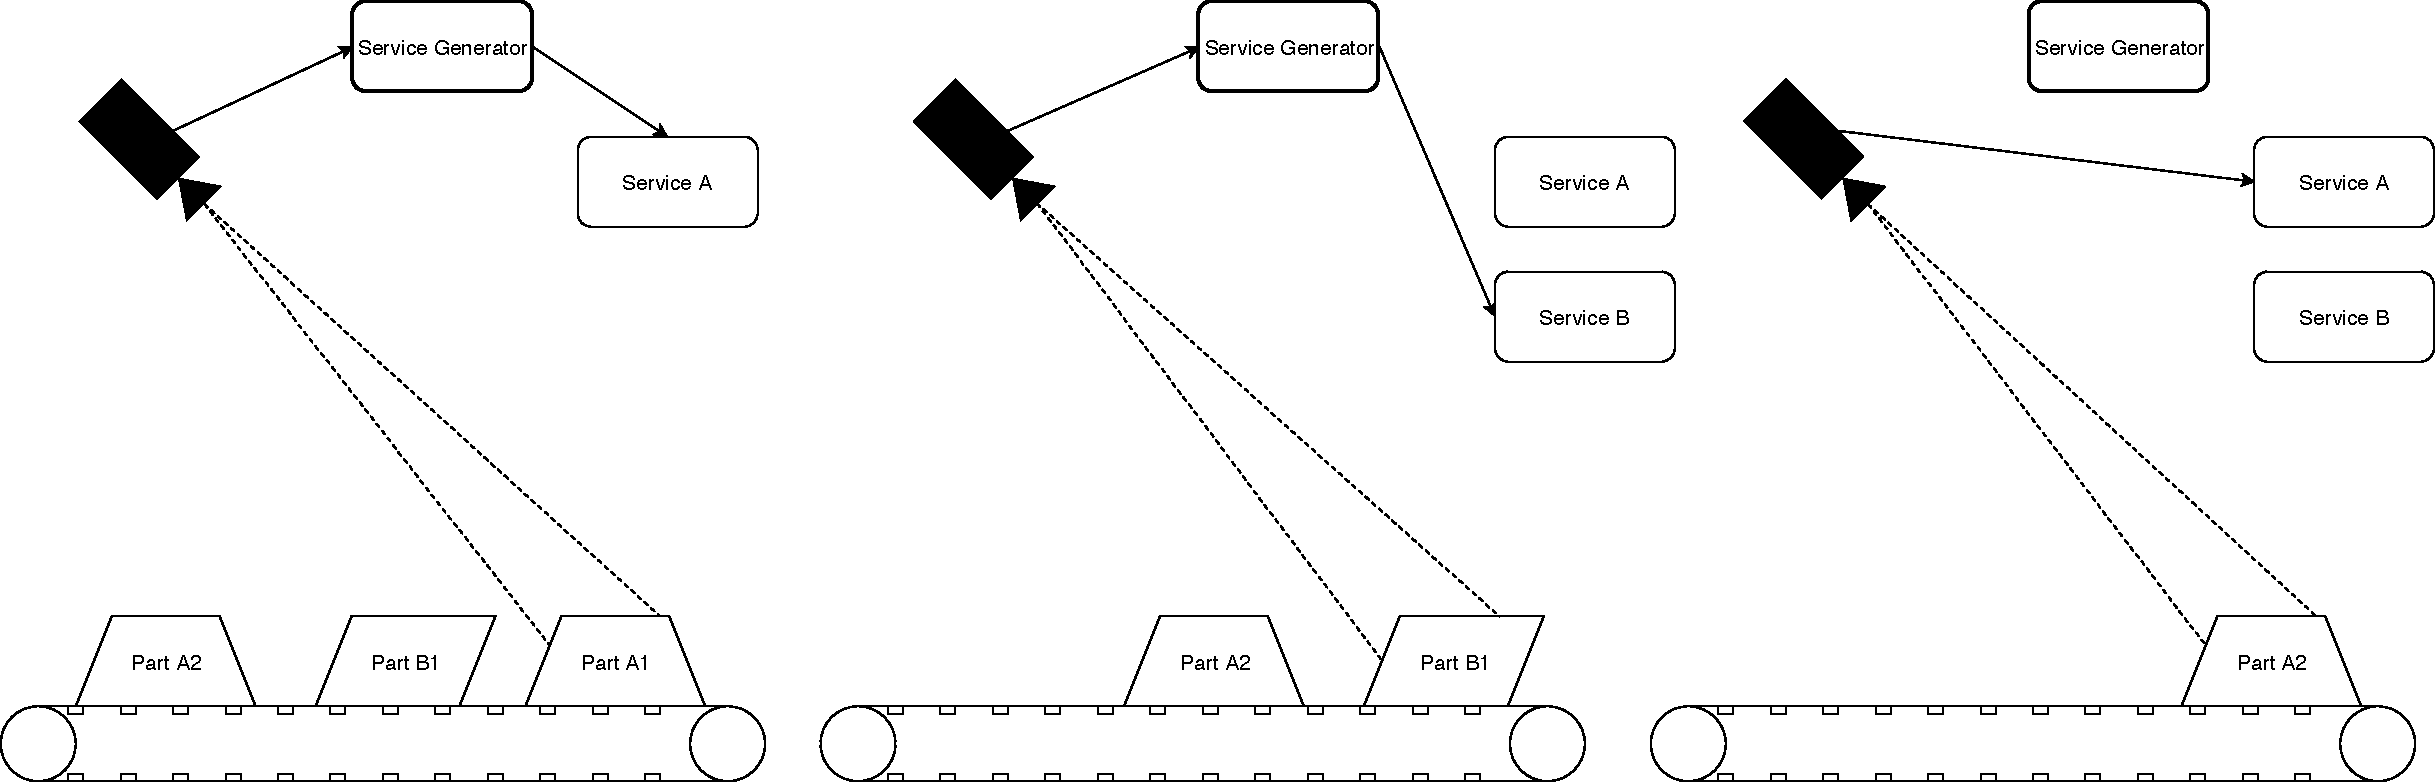
\includegraphics[width=\textwidth]{img/ServiceGenerationExample.pdf}
%     \caption{Service generation example in industrial context.}
%     \label{fig:ServiceGenExa}
% \end{figure}